% Paper II mechanism -- legitimacy-gated learning (clean grid, no overlaps).
% Compile: pdflatex fig1_mechanism.tex
\documentclass[border=7pt]{standalone}
\usepackage{amsmath,amssymb,bm}
\usepackage{tikz}
\usetikzlibrary{arrows.meta,positioning,fit,backgrounds,calc}
\begin{document}
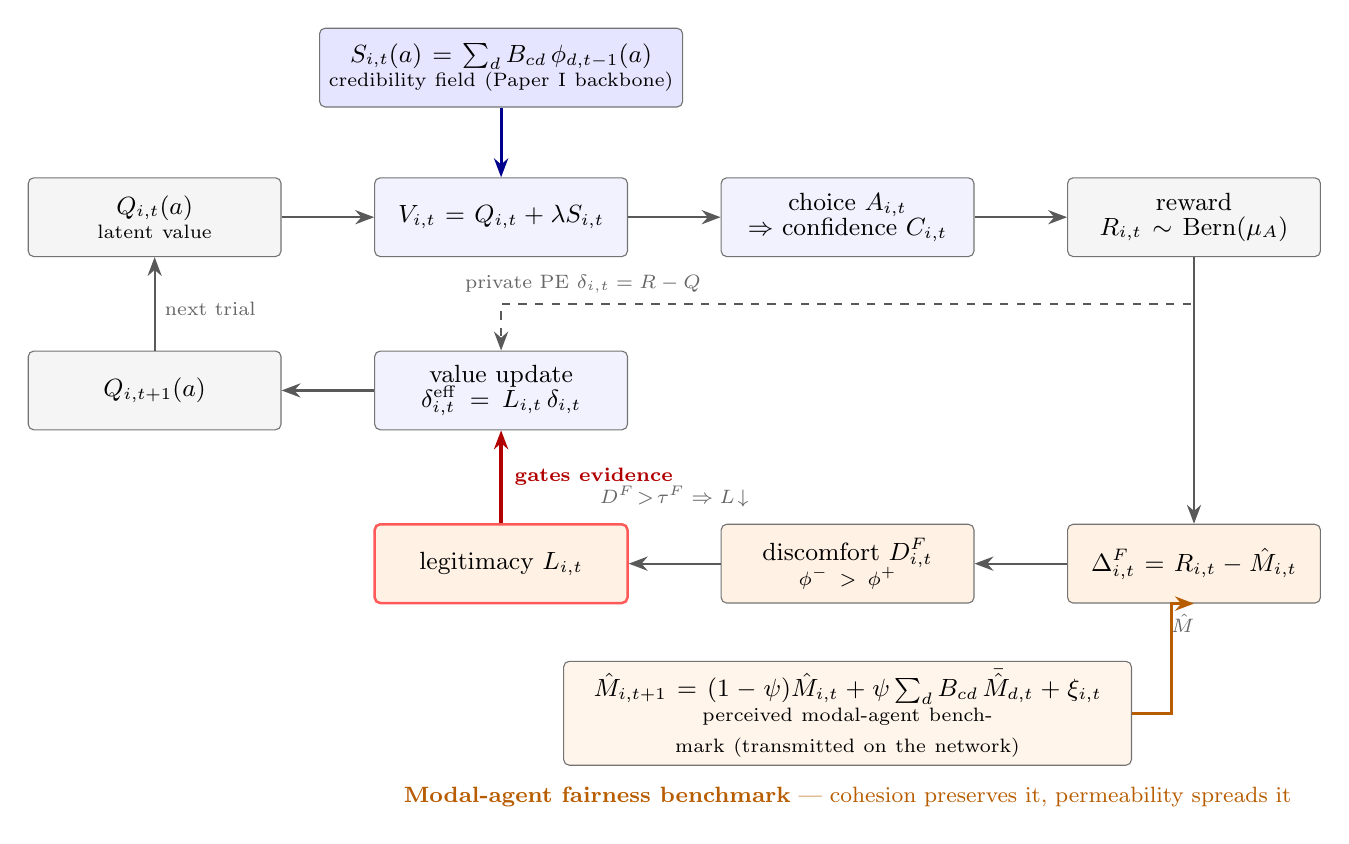
\begin{tikzpicture}[
  font=\small, >={Stealth[length=2.4mm]},
  box/.style={draw=black!55,rounded corners=2pt,align=center,
              minimum height=10mm,text width=30mm,inner sep=3pt},
  state/.style={box,fill=black!4},
  proc/.style={box,fill=blue!5},
  fair/.style={box,fill=orange!10},
  flow/.style={->,thick,black!65},
  gate/.style={->,line width=1.2pt,red!70!black},
  soc/.style={->,line width=1.1pt,orange!72!black},
  lbl/.style={font=\scriptsize,black!60},
]
% ===== grid (cm). columns x = 0, 4.4, 8.8, 13.2 ; rows y = 0, -2.2, -4.4, -6.2
\node[state] (Q)  at (0.0, 0.0) {$Q_{i,t}(a)$\\[-2pt]\scriptsize latent value};
\node[proc]  (V)  at (4.4, 0.0) {$V_{i,t}=Q_{i,t}+\lambda S_{i,t}$};
\node[proc]  (CH) at (8.8, 0.0) {choice $A_{i,t}$\\[-2pt]$\Rightarrow$ confidence $C_{i,t}$};
\node[state] (R)  at (13.2,0.0) {reward\\[-2pt]$R_{i,t}\sim\mathrm{Bern}(\mu_{A})$};
\node[box,fill=blue!10,text width=44mm] (S) at (4.4, 1.9)
     {$S_{i,t}(a)=\sum_d B_{cd}\,\phi_{d,t-1}(a)$\\[-2pt]\scriptsize credibility field (Paper~I backbone)};

% update lane (y=-2.2)
\node[proc]  (UPD) at (4.4,-2.2) {value update\\[-2pt]$\delta^{\mathrm{eff}}_{i,t}=L_{i,t}\,\delta_{i,t}$};
\node[state] (QN)  at (0.0,-2.2) {$Q_{i,t+1}(a)$};

% legitimacy lane (y=-4.4): L directly below UPD
\node[fair,draw=red!65,line width=0.9pt] (L) at (4.4,-4.4) {legitimacy $L_{i,t}$};
\node[fair] (DF)  at (8.8,-4.4) {discomfort $D^F_{i,t}$\\[-2pt]\scriptsize $\phi^-\!>\!\phi^+$};
\node[fair] (DFd) at (13.2,-4.4){$\Delta^F_{i,t}=R_{i,t}-\hat M_{i,t}$};

% benchmark (y=-6.2)
\node[box,fill=orange!8,text width=70mm] (MH) at (8.8,-6.3)
     {$\hat M_{i,t+1}=(1-\psi)\hat M_{i,t}+\psi\sum_d B_{cd}\,\bar{\hat M}_{d,t}+\xi_{i,t}$
      \\[-2pt]\scriptsize perceived modal-agent benchmark (transmitted on the network)};

% ===== value/choice flow =====
\draw[flow] (Q)  -- (V);
\draw[flow] (V)  -- (CH);
\draw[flow] (CH) -- (R);
\draw[soc,blue!55!black] (S) -- (V);

% private prediction error: reward -> update, clean band at y=-1.1
\draw[flow,dashed] (R.south) |- (7.0,-1.1) -| (UPD.north)
      node[pos=0.30,above,lbl]{private PE $\delta_{i,t}=R-Q$};

% update -> next value -> recurrence (clean far-left vertical)
\draw[flow] (UPD) -- (QN);
\draw[flow] (QN) -- node[right,lbl,pos=0.45]{next trial} (Q);

% fairness lane, right-to-left
\draw[flow] (R)  -- (DFd);
\draw[flow] (DFd) -- (DF);
\draw[flow] (DF) -- (L);
\node[lbl] at (6.6,-3.55) {$D^F\!>\!\tau^F\Rightarrow L\!\downarrow$};

% benchmark feeds the discrepancy
\draw[soc] (MH.east) -- ++(0.5,0) |- (DFd.south) node[pos=0.75,below,lbl]{$\hat M$};

% legitimacy GATES the update: clean vertical red arrow L -> UPD
\draw[gate] (L) -- node[right=1pt,font=\scriptsize\bfseries,red!70!black,pos=0.5]{gates evidence} (UPD);

% caption strip
\node[orange!72!black,font=\footnotesize,below=1.5mm of MH]
     {\textbf{Modal-agent fairness benchmark} --- cohesion preserves it, permeability spreads it};
\end{tikzpicture}
\end{document}
